\section{光滑解的失效}
\label{sec:cons-breakdown}

光滑解能活多久？特征线法可以回答这个问题：沿某条曲线把偏微分方程化成常微分方程。与第~\ref{chap:transport-equations}章的差别只在于曲线的速度依赖解。先假设$C^1$解存在，看它必须长什么样。

\paragraph{特征线是直线}
设$F\in C^2$，$u$是式~\eqref{eq:cons-law}的$C^1$解。从初始线上的点$(x_0,0)$出发，解常微分方程
\[
  x'(t)=F'\bigl(u(x(t),t)\bigr),\qquad x(0)=x_0 .
\]

沿这条曲线对$u$求导，再用式~\eqref{eq:cons-quasilinear}，得到
\[
  \frac{\mathrm{d}}{\mathrm{d}t}u(x(t),t)
  =\partial_tu+x'(t)\,\partial_xu
  =\partial_tu+F'(u)\,\partial_xu=0 .
\]

所以$u$沿曲线不变，始终等于$u_0(x_0)$。这样一来$x'(t)=F'(u_0(x_0))$是常数，曲线是一条直线。记
\begin{equation}
  a(x_0)=F'(u_0(x_0)),\qquad X_t(x_0)=x_0+a(x_0)\,t ,
  \label{eq:cons-characteristic}
\end{equation}
这些直线就是\term{特征线}（characteristic curve），$a(x_0)$是它的速度。解沿特征线保持常值：
\begin{equation}
  u\bigl(X_t(x_0),t\bigr)=u_0(x_0).
  \label{eq:cons-implicit}
\end{equation}

Burgers方程的$a=u_0$，特征线为$x=x_0+u_0(x_0)t$。下面的例子贯穿全章：
\begin{equation}
  u_0(x)=\frac{1}{1+x^2}.
  \label{eq:cons-bump}
\end{equation}

图~\ref{fig:cons-speed-arrows}把这条特征线翻译成波形的运动：曲线上的每个点水平移动，移动距离等于自己的高度。峰顶$x_0=0$、$u=1$的点在$t=1$移到$x=1$。右侧$x_0=2$、$u=1/5$的点只移到$x=2.2$。峰的右侧高处追赶低处，波形变陡；左侧高处离开低处，波形变缓。

\begin{BookInlineFigure}
  \centering
  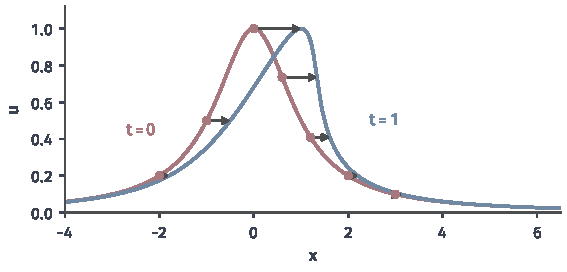
\includegraphics[width=96mm]{figures/06-differential-equations/02-partial-differential-equations/matplotlib/cons-speed-arrows/figure.pdf}
  \caption{Burgers方程中波形的水平移动。红线是初值~\eqref{eq:cons-bump}，红点是几个初始点，黑色箭头的长度等于该点的高度，蓝线是$t=1$的波形。峰的右侧被压陡，左侧被拉缓。}
  \label{fig:cons-speed-arrows}
\end{BookInlineFigure}

\paragraph{特征线相交与斜率爆炸}
斜率会变成多大？对式~\eqref{eq:cons-implicit}关于$x_0$求导，利用$\partial_{x_0}X_t=1+a'(x_0)t$，得到
\[
  \partial_xu\bigl(X_t(x_0),t\bigr)\,\bigl(1+a'(x_0)\,t\bigr)=u_0'(x_0).
\]

除过去，就是沿特征线的斜率公式：
\begin{equation}
  \partial_xu\bigl(X_t(x_0),t\bigr)=\frac{u_0'(x_0)}{1+a'(x_0)\,t}.
  \label{eq:cons-gradient}
\end{equation}

分母有直接的几何含义。$a'(x_0)$度量相邻特征线的速度差，两条相邻特征线的间距按因子$1+a'(x_0)t$变化。$a'<0$时，后面的特征线比前面的快，间距不断缩小；到$t=-1/a'(x_0)$，间距缩成零，分母为零，斜率发散。$a'>0$时间距增大，斜率随时间衰减。

在图~\ref{fig:cons-char-bump}中，初值峰右侧出发的特征线彼此靠拢，红色曲线是它们的包络，包络的尖点就是最早相交的位置。下面的例子算出这个点。

\begin{BookInlineFigure}
  \centering
  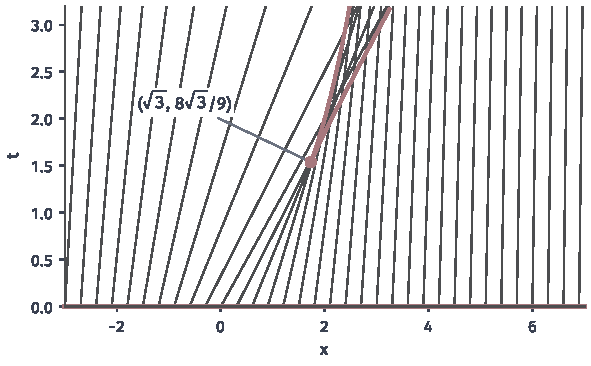
\includegraphics[width=100mm]{figures/06-differential-equations/02-partial-differential-equations/matplotlib/cons-char-bump/figure.pdf}
  \caption{初值~\eqref{eq:cons-bump}的特征线（深灰）。红色粗线是初始线，红色曲线是特征线的包络$t=-1/u_0'(x_0)$，$x=x_0+u_0(x_0)t$，它的尖点（红点）是特征线最早相交的位置。}
  \label{fig:cons-char-bump}
\end{BookInlineFigure}

\begin{example}[最早的相交点]
Burgers方程的$a=u_0$，取初值~\eqref{eq:cons-bump}。分母最早为零的特征线，出发点使$u_0'$最负。求导得
\[
  u_0'(x)=-\frac{2x}{(1+x^2)^2},\qquad u_0''(x)=\frac{6x^2-2}{(1+x^2)^3}.
\]

令$u_0''=0$，在$x>0$一侧得到$x_0=1/\sqrt{3}$。在这一点，
\[
  u_0(x_0)=\frac34,\qquad u_0'(x_0)=-\frac{2/\sqrt{3}}{(4/3)^2}=-\frac{3\sqrt{3}}{8}.
\]

于是最早的相交时刻和位置是
\[
  T^{*}=-\frac{1}{u_0'(x_0)}=\frac{8\sqrt{3}}{9}\approx1.54,\qquad
  x^{*}=x_0+\frac34T^{*}=\sqrt{3}.
\]
\end{example}

\paragraph{光滑解的寿命}
上面的计算是在假设解存在的前提下进行的。下面的定理确切地说明：相交时刻之前解存在且唯一，到了相交时刻不能再以$C^1$的方式继续。

\begin{theorem}[光滑解的寿命]
\label{thm:cons-lifespan}
设$F\in C^2(\mathbb{R})$，$u_0\in C^1(\mathbb{R})$，$u_0$与$u_0'$有界。记$a=F'\circ u_0$，$m=\inf_{\mathbb{R}}a'$。
\begin{enumerate}
  \item 若$m\geq0$，问题~\eqref{eq:cons-law}、\eqref{eq:cons-initial}在$\mathbb{R}\times[0,\infty)$上有唯一的$C^1$解。
  \item 若$m<0$，令
  \begin{equation}
    T^{*}=-\frac{1}{m},
    \label{eq:cons-breaking-time}
  \end{equation}
  此时问题在时间段$[0,T^{*})$上有唯一的$C^1$解，解的值保持在$[\inf u_0,\sup u_0]$内。当$t\uparrow T^{*}$时，$\sup_x\lvert\partial_xu(x,t)\rvert\to\infty$。对任何$T>T^{*}$，$\mathbb{R}\times[0,T]$上不存在$C^1$解；若下确界$m$在某点取到，$T=T^{*}$时同样不存在。
\end{enumerate}
\end{theorem}

\begin{proof}
记$T_0=\infty$（$m\geq0$时）或$T_0=T^{*}$（$m<0$时）。先看映射$X_t$。对$0\leq t<T_0$，
\[
  \partial_{x_0}X_t=1+a'(x_0)\,t\geq1+\min(m,0)\,t>0 .
\]
导数有正的下界，所以$X_t$严格递增，且把$\mathbb{R}$映满$\mathbb{R}$，是$C^1$同胚。

唯一性：设$u$是$\mathbb{R}\times[0,T_0)$上的$C^1$解。前面已经说明，$u$沿式~\eqref{eq:cons-characteristic}的直线不变。这些直线在$t$时刻覆盖整条实轴，所以$u$的值被式~\eqref{eq:cons-implicit}完全确定。

存在性：令$\xi(x,t)$是方程$X_t(\xi)=x$的解。由隐函数定理，$\xi\in C^1$，并且
\[
  \partial_x\xi=\frac{1}{1+a'(\xi)\,t},\qquad
  \partial_t\xi=-\frac{a(\xi)}{1+a'(\xi)\,t}.
\]

定义$u(x,t)=u_0(\xi(x,t))$。它在$t=0$取$u_0$，并且$F'(u)=a(\xi)$，所以
\[
  \partial_tu+F'(u)\,\partial_xu
  =u_0'(\xi)\bigl(\partial_t\xi+a(\xi)\,\partial_x\xi\bigr)=0 .
\]
第一条结论与第二条的存在性就此成立。$u$的值都是$u_0$的值，所以落在$[\inf u_0,\sup u_0]$内。

斜率发散：设$m<0$。取点列$x_n$使$a'(x_n)\to m$。记$C=\max\lvert F''\rvert$，最大值取在$u_0$值域的闭包上，它是紧集，且$C>0$（否则$a'\equiv0$）。由$a'=F''(u_0)u_0'$，当$n$充分大时
\[
  \lvert u_0'(x_n)\rvert\geq\frac{\lvert a'(x_n)\rvert}{C}\geq\frac{\lvert m\rvert}{2C}.
\]

对固定的$t<T^{*}$，有$1+mt>0$，且$n\to\infty$时$1+a'(x_n)t\to1+mt$。取$n$充分大，使$1+a'(x_n)t\leq2(1+mt)$，由式~\eqref{eq:cons-gradient}，
\[
  \sup_x\lvert\partial_xu(x,t)\rvert\geq\frac{\lvert m\rvert}{4C\,(1+mt)}.
\]
令$t\uparrow T^{*}$，右端趋于无穷。

不可延拓：设$u$是$\mathbb{R}\times[0,T]$上的$C^1$解，$T>T^{*}$。由$m<-1/T$，存在$x_0$使$a'(x_0)<-1/T$；若下确界在某点取到且$T=T^{*}$，就取该点。令$t_1=-1/a'(x_0)\in(0,T]$，此时$a'(x_0)\neq0$，从而$u_0'(x_0)\neq0$。

前面的推导对解存在的整个时间段成立，于是在$t=t_1$时
\[
  \partial_xu\bigl(X_{t_1}(x_0),t_1\bigr)\,\bigl(1+a'(x_0)\,t_1\bigr)=u_0'(x_0).
\]
左端的第二个因子为零，右端不为零，矛盾。
\end{proof}

对Burgers方程，$a'=u_0'$，$T^{*}=-1/\inf u_0'$。特别地，有界的$C^1$初值（导数有界）给出整体$C^1$解，当且仅当$u_0$单调不减。定理中的条件各有作用：$u_0'$有界保证$m$有限，否则$T^{*}$可以为零；$F''$非零才让速度随$u$变化，线性通量的$a'\equiv0$，永远不会相交。

有界性和光滑性是分开的两件事。第~\ref{chap:ordinary-differential-equations}章的爆炸是解的值趋于无穷；这里相反，解的值始终在初值范围内，发散的是导数。图~\ref{fig:cons-gradient-blowup}显示，初值~\eqref{eq:cons-bump}的压缩侧斜率在$T^{*}$发散，膨胀侧斜率逐渐衰减，而最大值始终为$1$。

\begin{BookInlineFigure}
  \centering
  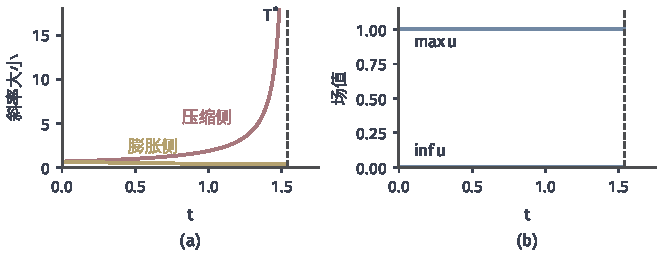
\includegraphics[width=112mm]{figures/06-differential-equations/02-partial-differential-equations/matplotlib/cons-gradient-blowup/figure.pdf}
  \caption{初值~\eqref{eq:cons-bump}的斜率与场值。(a)红线是压缩侧的最大下降斜率$\max_{x_0}(-u_0'/(1+tu_0'))$，黄线是膨胀侧的最大上升斜率，虚线是$T^{*}$。(b)场值的上界和下确界（蓝）不随时间变化。}
  \label{fig:cons-gradient-blowup}
\end{BookInlineFigure}

\paragraph{相交之后发生了什么}
定理说的是映射$X_t$的单调性。图~\ref{fig:cons-fold-map}画出$x_0\mapsto X_t(x_0)$在三个时刻的形状：$T^{*}$之前严格递增，$T^{*}$时出现水平切点，之后出现折叠，同一个$x$有三个原像，也就是有三条特征线到达同一点，各自带来不同的值。

\begin{BookInlineFigure}
  \centering
  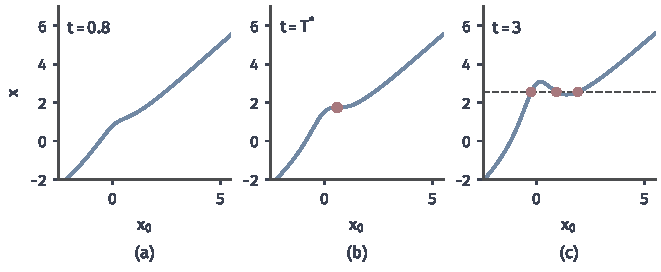
\includegraphics[width=112mm]{figures/06-differential-equations/02-partial-differential-equations/matplotlib/cons-fold-map/figure.pdf}
  \caption{初值~\eqref{eq:cons-bump}的映射$X_t$。(a)$t=0.8$，严格递增。(b)$t=T^{*}$，红点是水平切点$(1/\sqrt{3},\sqrt{3})$。(c)$t=3$，映射折叠，虚线$x=2.55$与曲线有三个交点（红点）。}
  \label{fig:cons-fold-map}
\end{BookInlineFigure}

把折叠的结果画成波形，就是图~\ref{fig:cons-steepening}(b)：曲线翻转，成为多值的。水面的波可以卷起来，同一个$x$上有几层水；密度却不能，同一时刻同一地点只有一个车流密度。所以$T^{*}$之后，式~\eqref{eq:cons-implicit}不再给出一个函数。

\begin{BookInlineFigure}
  \centering
  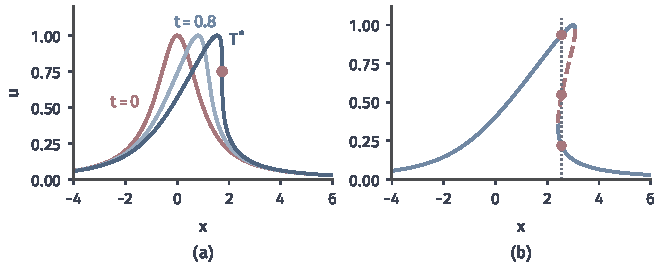
\includegraphics[width=112mm]{figures/06-differential-equations/02-partial-differential-equations/matplotlib/cons-steepening/figure.pdf}
  \caption{波形的变陡与翻转。(a)红线是$t=0$，蓝色由浅到深是$t=0.8$和$t=T^{*}$，红点是斜率首次为无穷的位置$(\sqrt{3},3/4)$。(b)$t=3$时沿特征线算出的图像，红色虚线是翻转部分，竖直点线$x=2.55$上有三个值。}
  \label{fig:cons-steepening}
\end{BookInlineFigure}

第~\ref{chap:transport-equations}章的轨迹不会相交，原因是给定的Lipschitz速度场让常微分方程的解唯一，两条轨迹不能在同一时刻到达同一点。这里两条特征线到达同一点时带着不同的场值，也就有不同的速度，它们不是同一个速度场下的轨迹，唯一性定理管不到它们。速度依赖解，正是相交的来源。

\paragraph{斜坡：所有特征线同时汇聚}
还有一个算起来更简单的初值：
\begin{equation}
  u_0(x)=\begin{cases}1,&x<0,\\1-x,&0\leq x\leq1,\\0,&x>1.\end{cases}
  \label{eq:cons-ramp}
\end{equation}

它只是Lipschitz连续，但沿特征线的计算不受影响。在$(0,1)$上$a'=-1$，从那里出发的特征线$x=x_0+(1-x_0)t$全部在$(1,1)$汇聚，$T^{*}=1$。反解出$x_0=(x-t)/(1-t)$，得到$t<1$时的解
\begin{equation}
  u(x,t)=\frac{1-x}{1-t},\qquad t\leq x\leq1,
  \label{eq:cons-ramp-solution}
\end{equation}
其余区域取常值$1$或$0$。第~\ref{sec:cons-weak}节将接着算出$t>1$时的解，这时解必须带一个间断。
